\chapter{Проектиране на модулите системата}
\section{Изискване към функционалните възможности на системата}
В настоящата дипломна работа е представена платформено независима
система за езиково обучение. Създадената система бе именувана
"`Spellbook"'(книга с вълшебства/игра на думи с английските думи
"`spell"'(сричам) и "`book"'(книга/учебник)). За съхранение на
информацията си локално приложението използва релационна система за
управление на база данни(РСУДБ), а именно H2 Database. Приложението
поддържа и синхронизиране на локалната база данни с централна такава
през интернет. Централната база данни се съхранява в MySQL.

Spellbook е десктоп приложение, реализирано посредством библиотеката
Swing на Java Standard Edition. Функционалността на приложението е
разделена модулно, за да се окуражи преизползването на части от кода
му и в други проекти. Например лесно би било да се създаде уеб версия
на приложението написана на Java - единственият нов код в нея би бил
кода на графичния потребителски интерфейс. Най-общо системата има 3
слоя - потребителски интерфейс, слой на услуги(сервизен слой/service
layer) и база данни.

Стремейки се да бъде една модерна система за езиково обучение
Spellbook предлага на своите потребители атрактивен графичен интерфейс,
разнообразни образователни модули и много интересни възможности като
интеграция със системния клипборд, възможност за автоматично сваляне
на речници, проверка на правопис, възможност за промяна на въшния
вид. 

Една от най-важните характеристи на приложението е възможността
потребителите му активно да допринасят за развитието на речниковата
база, посредством добавянето на нови думи в нея и корекцията на
съществуващите. 

Обърнато е внимание на минимизирането на използваните ресурси, както и
на максимизирането на производителността. Използването на релационна
база данни за съхранението на речниците например, прави търсенето в
сравнително голям речник почти моментално. 

Диагностиката на проблеми, възникнали по време на работата на
приложението е много лесна благодарение на подробния журнал, който
води приложението по време на своето изпълнение, както и да описателните
съобщения за грешки, което то използва. 

Макар, че Spellbook е платформено независим - дистрибутивите чрез,
които се разпространява са специфични за по-популярните операционни
системи, за да се улесни процеса на инсталацията на приложението върху
тях.  
\section{Архитектура на системата}
Най-общо системата представлява едно класическо трислойно приложение -
потребителски интерфейс, бизнес слой и база данни. Потребителя
комуникира с приложението единствено през потребителския интерфейс,
който пък комуникира с бизнес слоя и реагира на действията на
потребителя. Бизнес слоя евентуално(но не задължително) комуникира с
базата данни и данни достъпни посредством интернет.

\begin{figure}[htbp]
  \caption{Обобщена архитектура}
  \centering
  \includegraphics[width=80mm, height=120mm]{images/basic_arch.png}
\end{figure}

Потребителският интерфейс е базиран на библиотеката Swing, като освен
стандартните компоненти са добавени и тези от популярната библиотека
JIDE OSS. Базата данни е H2 във вграден режим - това значи, че тя
работи в адресното пространство на самото приложение, а не като
сървър. Това лимитира достъпа до нея само до един процес, но увеличава
многократно производителността и.

\begin{figure}[htbp]
  \caption{Поток на контрол}
  \centering
  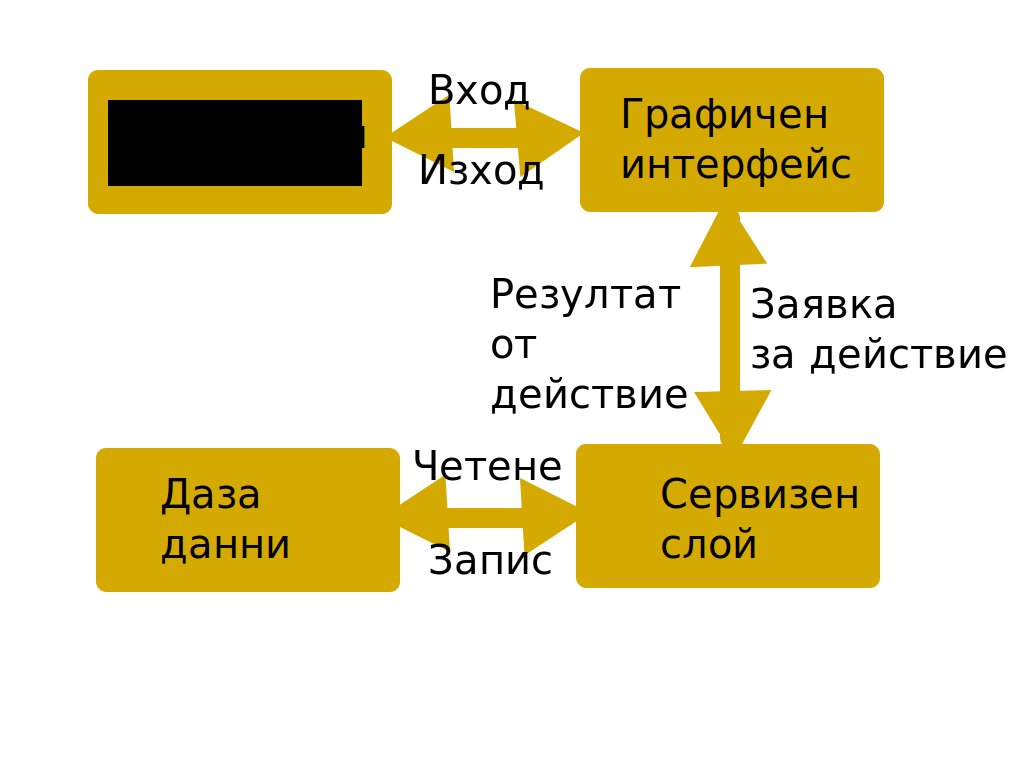
\includegraphics[width=80mm, height=120mm]{images/flow.png}
\end{figure}
\section{Възможности на системата}
\subsection{Речник}
Системата може да функционира като речник - поддържат се точно търсене
на думи, приблизително търсене на думи, търсене на думи в
комплементарен речник, история на търсените думи, търсене активирано
чрез копиране на дума в клипборда. 

Освен това речниковият фонд е разширяем от потребителите, а не е
фиксиран. Те могат лесно да добавят нови думи и да редактират
съществуващите. Речниковата база данни е достъпна отделно от приложението
и при желание други проекти могат да я ползват също.
\begin{figure}[htbp]
  \caption{Работа на речника}
  \centering
  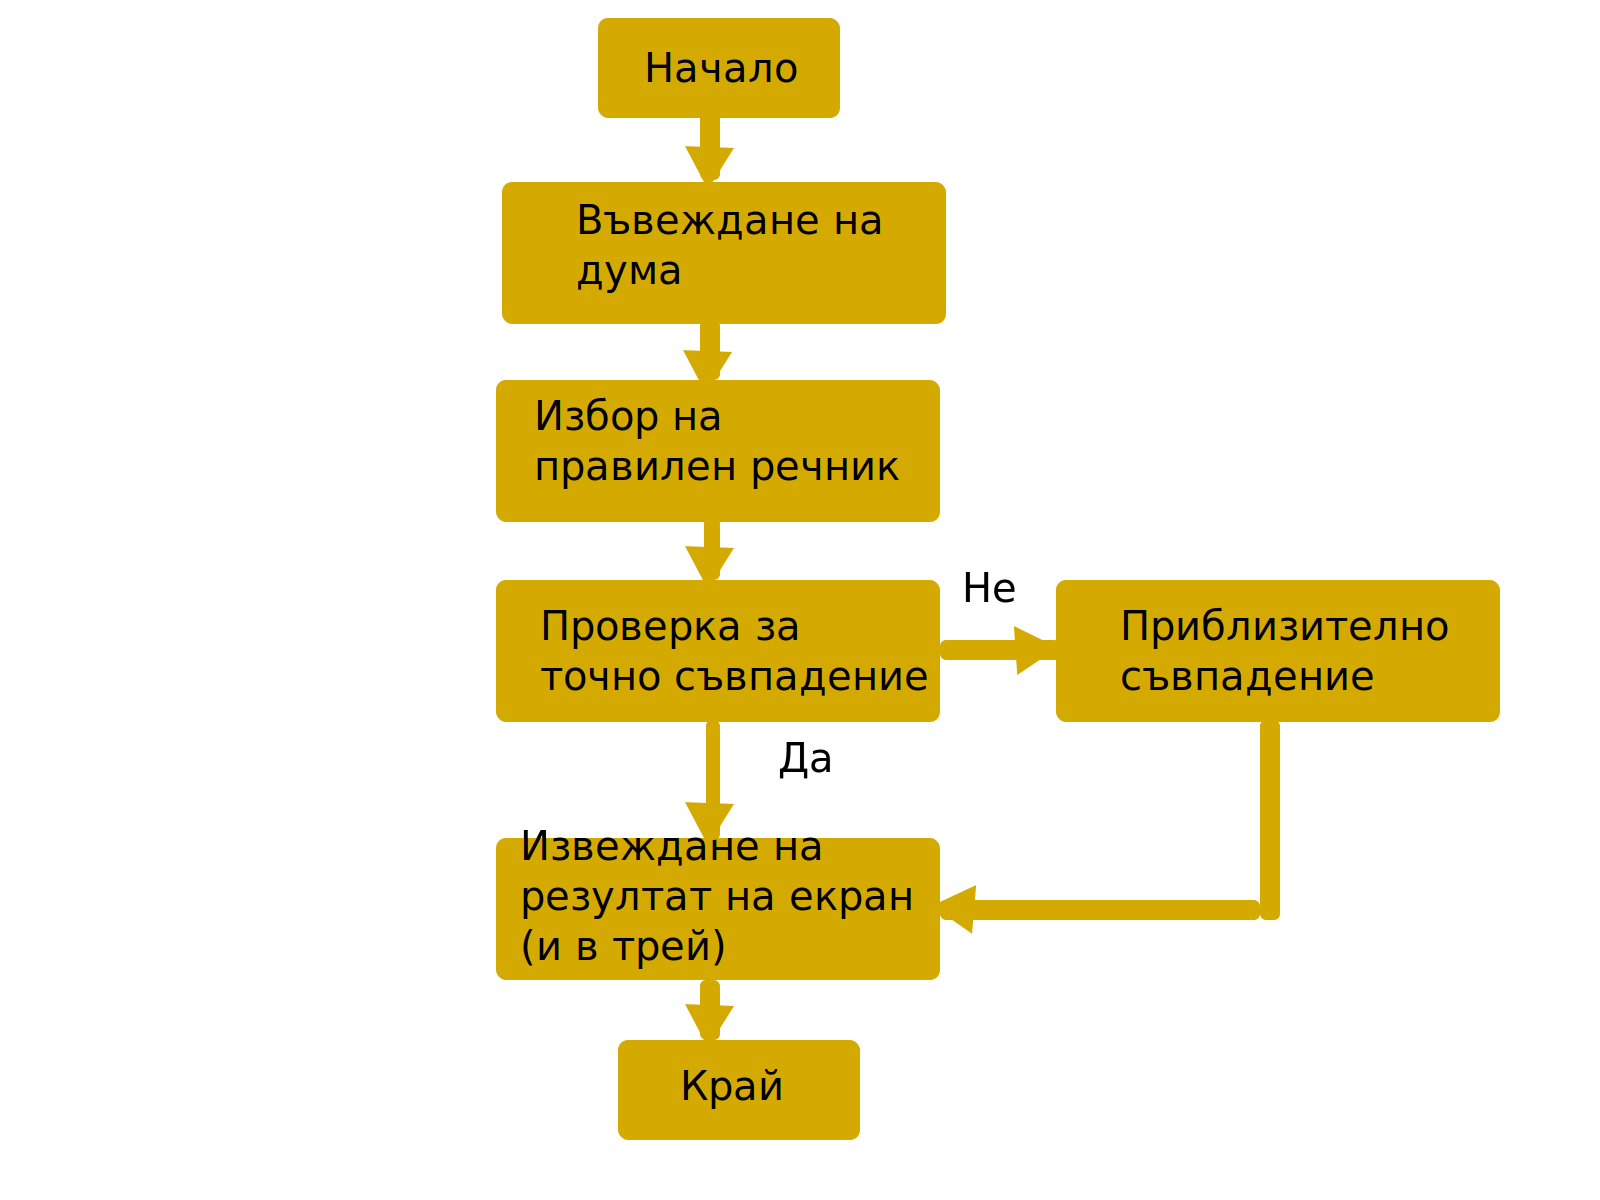
\includegraphics[width=80mm, height=120mm]{images/dictionary_flow.png}
\end{figure}

\subsection{Изпит}
Системата включва модул изпит, чрез който потребителите могат да
упражняват и разширяват познанията си по даден език. Изпитът предлага
различни нива на сложност генерирани интелигентно, посредством
статистически анализ на езика. Често срещаните думи са маркират като
лесни и обратното. Изпитният модул, накрая на всеки изпит, предлага на
потребителя подробна статистика за неговото представяне и възможност
да запази резултата си за бъдеща справка.

\begin{figure}[htbp]
  \caption{Работа на изпита}
  \centering
  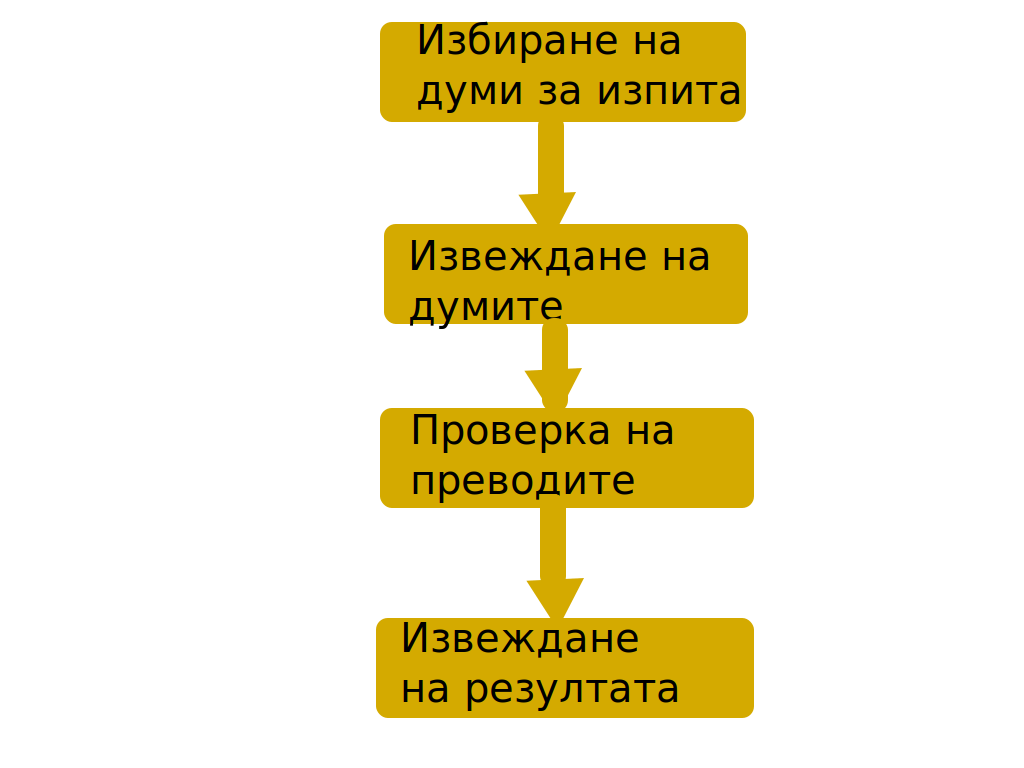
\includegraphics[width=80mm, height=120mm]{images/exam_flow.png}
\end{figure}

\subsection{Учене на думи}
Системата включва модул за изучаване на думи, подходящ за ученици в
езикови гимназии и студенти във филологически специалности. Той им
предоставя възможност да създадат набор от думи, които искат да
изучават активно. Функционалността наподобява локализиран изпит. В
бъдеще системата може да предлага по подразбиране някои готови набори
от думи - например животни, плодове, зеленчуци(думи подходящи за
начинаещи), както и думи за изпита САТ1 например(думи подходящи за
напреднали или целево изучаващи).
\subsection{Игри}
Популярно мнение, е че материал се усвоява по-лесно(особено от
децата), когато е предложен във формата на игри. В тази връзка
системата има секция с образователни игри. Понастоящем там има само
една игра - "`Бесеница"'. Планът е, обаче, в бъдеще секцията да бъде
разширена с други игри, като например скрабъл(scrabble) и асоциации.
\subsubsection{Бесеница}
Системата включва игра "`Бесеницата"' целта, на която е проста - да се
познае определена дума по значението и. Потребителят има право да
въвежда по една буква или цялата дума, ако прецени, че я е разгадал. В
началото на играта потребителят трябва да избере два езика и трудност
подобно на изпитния модул. След няколко неуспешни опита потребителят
губи играта(или казано на жаргона и - "`бива обесен"'). 
\subsection{Проверка на правописа}
Системата предлага модул за проверка на правописа, който в един
образователен курс може да се използва за моментална проверка на
дигитализирани диктовки, например. Модулът реализира ефективен
алгоритъм за определяне на правилността на думите и предлага корекции
на грешните думи. 
\subsection{Синхронизация с централна база данни}
Spellbook е само едната страната на монетата. В паралелна дипломна
работа се разработва уеб версия на системата, която притежава
централизирана база данни. Една от най-интересните възможните на
Spellbook е именно сихронизирането с тази централна база данни - така
потребителите ще могат да споделят помежду си своите промени.

\begin{figure}[htbp]
  \caption{Синхронизация}
  \centering
  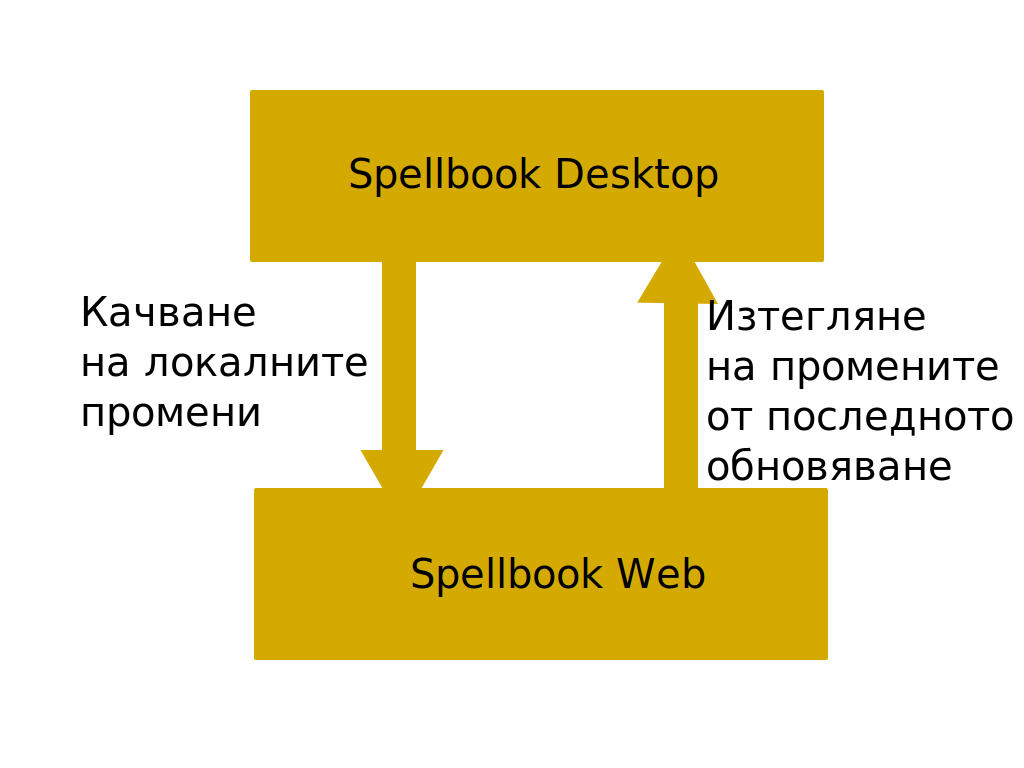
\includegraphics[width=80mm, height=120mm]{images/sync_flow.png}
\end{figure} 
\section{Структура на Maven проекта}
В духа на съвременните Java технологии и тенденции проектът използва
Maven 2 като инструмент за изграждане и поддържане. В тази връзка той
вътрешно е разделен на няколко maven модула, има зависимости към някои
външния Java библиотеки(терминът в Maven е артефакт) и използва
няколко разширения(plugins) на Maven.
\subsection{Модули}
Приложението е разделено на четири Maven модула:
\begin{itemize}
\item \textbf{Ядро}

Тук се намира огромната част от бизнес логиката(слоя) на системата -
абстракцията над достъпа до базата данни, бизнес модела,
класовете-услуги за речника, изпита, проверката на правописа и модула
за учене на думи, преводача на потребителския интерфейс.

Модулите "`Swing компоненти"' и "`Потребителски интерфейс"' вътрешно
използват този модули. 
\item \textbf{Swing компоненти}

В този модул са дефинирани някои допълнителни Swing компоненти, които
се използват на различни места в приложението. Модулът се използва
вътрешно от модула "`Потребителски интерфейс"'.
\item \textbf{Помощни пособия}

Всякакви помощни класове, методи и код, който няма място в другите
модули е събран тук. Всички други модули го използват. Той не трябва
да използва никой от другите модули - в противен случай ще възникне
кръгова зависимост между модулите.
\item \textbf{Потребителски интерфейс}

Основната част от кода на потребителския интерфейс се намира в този
модул - главния прозорец на приложението, диалоговите прозорци на
всички инструменти и много други. Модулът вътрешно използва всички
други модули на приложението. Тук се намира и изпълнимият клас на
приложението SpellbookApp. 
\end{itemize}
\begin{figure}[htbp]
  \caption{Maven структура}
  \centering
  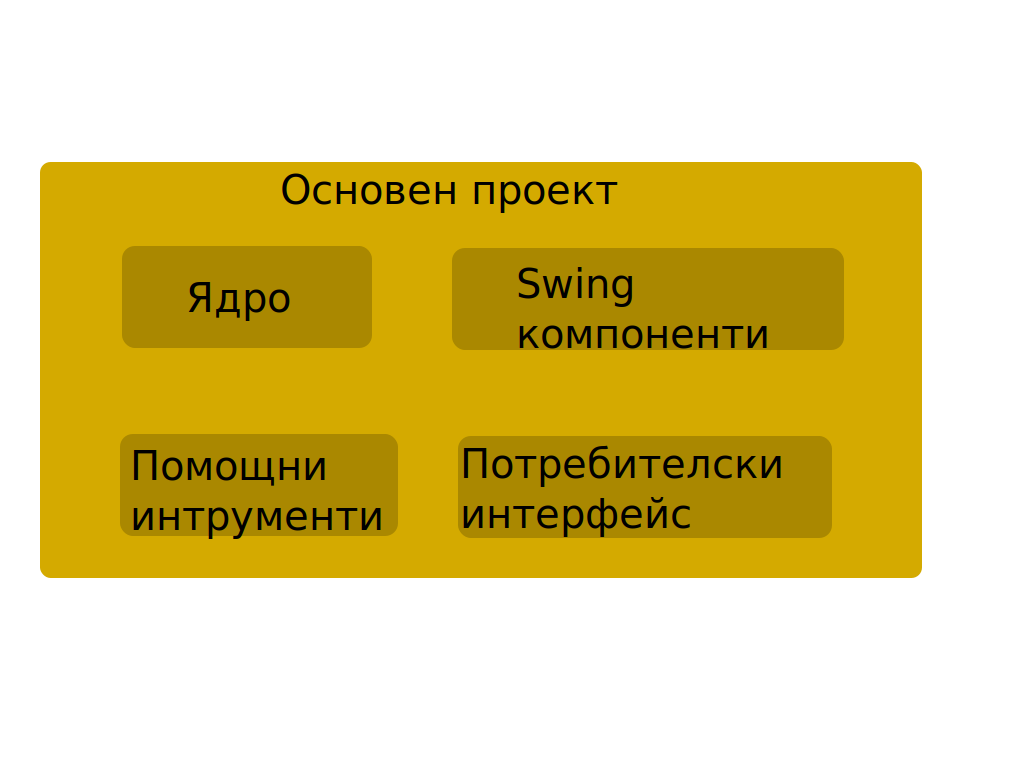
\includegraphics[width=80mm, height=120mm]{images/maven_modules.png}
\end{figure}
    
\subsection{Зависимости}
Проекта зависи от някои външни Java библиотеки, които добавят много
функционалност към стандартната библиотека на Java:

\begin{itemize}
  \item \textbf{Hibernate 3.5}

    Hibernate предоставя обектно-релационно преобразуване за
    приложението. Освен това актуалната версия на Hibernate 3.5
    имплементира спецификацията Java Persistence API 2.
  \item \textbf{H2 1.1.117}

    Базата данни H2 е написана изцяло на Java и работи като част от
    приложението в неговото адресно пространоство(вграден режим).
  \item \textbf{MySQL Java Connector 5.1.12}

    MySQL JDBC конектор - необходим за установяне на връзка с MySQL
    база данни от Java приложение.
  \item \textbf{Balloon tip 1.0}

    Swing библиотека, която реализира показването на балончета с
    информация. 
  \item \textbf{JIDE OSS 2.8.4}

    JIDE OSS е популярна Swing библиотеката, която подобрява някои от
    стандартните Swing компоненти и добавя много други нови компоненти.
  \item \textbf{MigLayout 3.7.1}

    Модерен layout manager за Swing. Позволява лесно създаване на
    елегантни потребителски интерфейси без употребата на графични
    дизайнери. Употребата му подобравя сериозно четимостта и
    качеството на кода, който генерира потребителския интерфейс.
  \item \textbf{SLF4J 1.5.8}

    Фасадна журнална библиотека за Java, подобна на Apache Commons. В
    приложението се използва в комбинация с Simple Log за генерирането
    на подробен журнал за работата му.
  \item \textbf{Ant 1.7.1}

    По принцип Ant е алтернативен инструмент на Maven за изграждане и
    управление на Java проекти. Тук, обаче, е използван заради
    възможността си да работи с tar и bzip2 архиви.
  \item \textbf{JUnit 4.7}

    Платформа за тестове.
\end{itemize}
\subsection{Пакетиране}

Maven посредством командата си \textbf{mvn package} може да създаде от
приложението jar файл. Да за бъде използваем той от потребителите,
обаче, е необходимо те да имат в своя класпът(classpath) всички зависимости на
приложението. Има два подхода за решаване на този проблем - единият е
приложението да се дистрибутира отделно от зависимостите си и те да
бъдат добавени в lib директория, която да бъде включвана автоматично в
класпътя. Предпочетен, обаче, беше друг вариант - приложението да бъде
пакетирано директно със зависимостите си, за да е по-лесно на крайните
потребители да работят с него. Maven прави тази задача много лесна
благодарение на разширението си assembly. За да се създаде jar файл,
който съдържа приложението и всичките му зависимости е необходимо
просто да бъде изпълнена командата:

\textbf{mvn assembly:assembly}

След изпълнението и в директорията target на проекта редом до файла
application-version.jar ще бъде и файла
application-version-jar-with-dependencies.jar.

Обикновените потребители не са особено запознати с това как да
стартират един jar файл, за това е добре крайната версия на продукта
да е допълнително пакетирана по начин, по който потребителите лесно да
боравят с нея. За GNU/Linux дистрибуциите това е пакет(RPM, DEB), за
Windows потребителите - инсталатор. Освен това трябва да включим и
изпълним файл за стартирането на приложението - exe в Windows и шел(shell)
скрипт за Unix подобните операционни системи. Шел скрипта най-общо
трябва да изпълнява просто следната команда:

\textbf{java -jar application.jar}

Дистрибутивът за Windows пък е създаден с популярната свободна
програма IzPack, която позволя да се създават инсталатори и изпълними
файлове за Java приложения. 

Тъй като никога не могат да бъдат покрити абсолютно всички операционни
системи приложението допълнително се разпространява и като обикновен
архив, който всички потребители могат да ползват без особено
затруднение. 

Текущите версии на всички дистрибутиви на системата са достъпни за
сваляне на официалната страница на проекта.
\section{Структура на базата данни}

Структурата на базата данни е генерирана от инструмента Liquibase. Той
бе предпочетен пред създаването на SQL скриптове на ръка заради
възможността му да следи ревизиите на базата данни, да инсталира
автоматично новите ревизии и да бъде изпълнявам автоматично от Maven
при компилиране. Това гарантира, че всички разработчици в даден момент
работят с актуалната версия на базата данни. Освен това Liquibase е
портативен - от неговия специален markup може да се генерира SQL за
различни релационни бази данни.

Таблицата \emph{Dictionaries} съдържа информация за наличните речници,
а таблицата \emph{Dictionary\_Entries} съдържа самите думи на
речниците. Таблиците \emph{Study\_Sets} и \emph{Study\_Set\_Entries} пък
съдържат информация за наборите от думи за учене и думите в тях. 

\begin{figure}[htbp]
  \caption{Структура на речниците и наборите от думи}
  \centering
  \includegraphics[width=90mm, height=160mm]{images/db_diagram.png}
\end{figure}

Таблицата \emph{Exam\_Score\_Entries} съдържа резултатите от положените
изпити. Съхранява се информация за процентната успеваемост, езика и
трудността на изпита, както и псевднима на положилия го.

\begin{figure}[htbp]
  \caption{Структура на резултатите от изпита}
  \centering
  \includegraphics[width=60mm, height=50mm]{images/exam_score_entries_diagram.png}
\end{figure}

В таблицата \emph{Rank\_Entries\_Table} пък се съхранявам
ранговете(оценките) на думите, които се използват в последствие от
изпитния модул. Таблицата е популирана от различни книги и честотата
на срещането на думи в тях е използвана за база на формиране на ранга
на всяка дума.

\begin{figure}[htbp]
  \caption{Структура на ранговете на думи}
  \centering
  \includegraphics[width=60mm, height=50mm]{images/rank_entries_table.png}
\end{figure}

Базата данни включва и няколко служебни таблици, които са свързани с
работата на инструмента Liquibase. Тяхната структура, обаче, не
преставлява интерес за приложението.

%%% Local Variables: 
%%% mode: latex
%%% TeX-master: "master"
%%% End: 
